\documentclass[11pt]{article}

\usepackage{geometry}
\usepackage{graphicx}
\usepackage{siunitx}
\usepackage{amsmath}
\usepackage{enumerate}
\usepackage{multirow}
\usepackage{indentfirst}
\usepackage{float}

\geometry{top=1.3in, bottom=1.3in, left=1.0in, right=1.0in}

\setlength{\parindent}{2em}

\newcommand{\e}[1]{\times10^{#1}}
\newcommand{\degree}{^\circ}

\linespread{1.3}

\begin{document}

\begin{titlepage}
\begin{center}
\vspace*{2cm}

\doublespacing
\rule{\linewidth}{0.3mm}

\textsc{
	\large
	UM-SJTU Joint Institute\\ 
	Physical Laboratory\\
	VP141
}

\rule{\linewidth}{0.3mm}


\vspace*{3.5cm}

{
\Large
\textsc{Laboratory Report}\\
}

\vspace*{0.2cm}

{
\large
\textsc{Exercise 4} \\
\textsc{Measurement of the Speed of Sound}
}

\end{center}

\vfill
\normalsize

\hspace*{1cm}
\begin{minipage}{0.4\textwidth}
\begin{tabular}{p{1.7cm}p{4cm}llll}
Name: &  Ren Wang \hspace*{0.6cm} {\fontspec{Hei}\selectfont 王韧} & ID: & 516370910177 & Group: & 11 \\
Name: &  Biyang Guo {\fontspec{Hei}\selectfont 郭铋扬} & ID: & 516370910246 & Group: & 11 \\
\multicolumn{6}{l}{Date: \today}
\end{tabular}
\end{minipage}

\end{titlepage}
\section{Introduction}
    The objective of the exercise is to measure the fluid viscosity, an important property of fluids, using Stoke's method.\\

    To analyze the free body diagram of a spherical object moving in a fluid, we find that the viscous force, the buoyancy force and the weight, where the first two forces act upwards and the last one  acts downwards.\\

    The magnitude of a drag force is related to the shape and speed of the objective as well as to the internal friction in the fluid. We use coefficient $\eta$ to quantify the internal friction in the fluid. Hence we build a model for the drag force (viscous force) in an infinite volume of a liquid.
    \[
        F_1=6\pi\eta vR
    \]
    The magnitude of the buoyancy force is
    \[
        F_2=\frac{4}{3}\pi R^3\rho_1g,
    \]
    where $\rho_1$ is the density of the fluid and g is the acceleration due to gravity. The weight of the object is
    \[
        F_3=\frac{4}{3}\pi R^3\rho_2g,    
    \]
    where $\rho_2$ is the density of the object. Since the three forces balance each other, then 
    \[
        F_1+F_2=F_3.
    \]
    Assuming that the object will be moving with constant speed $v_t$, we find from the equation that
    \[
        \eta=\frac{2}{9}gR^2\frac{\rho_2-\rho_1}{v_t}.
    \]

\section{Experimental setup}
    This exercise requires a Stokes' viscosity measurement device (see Figure \ref{apparatus}) with castor oil and some small metal balls. The experiment also requires devices including micrometer, calliper, densimeter, electronic scales, stopwatch, and thermometer.
    \begin{figure}[htbp]
        \centering
        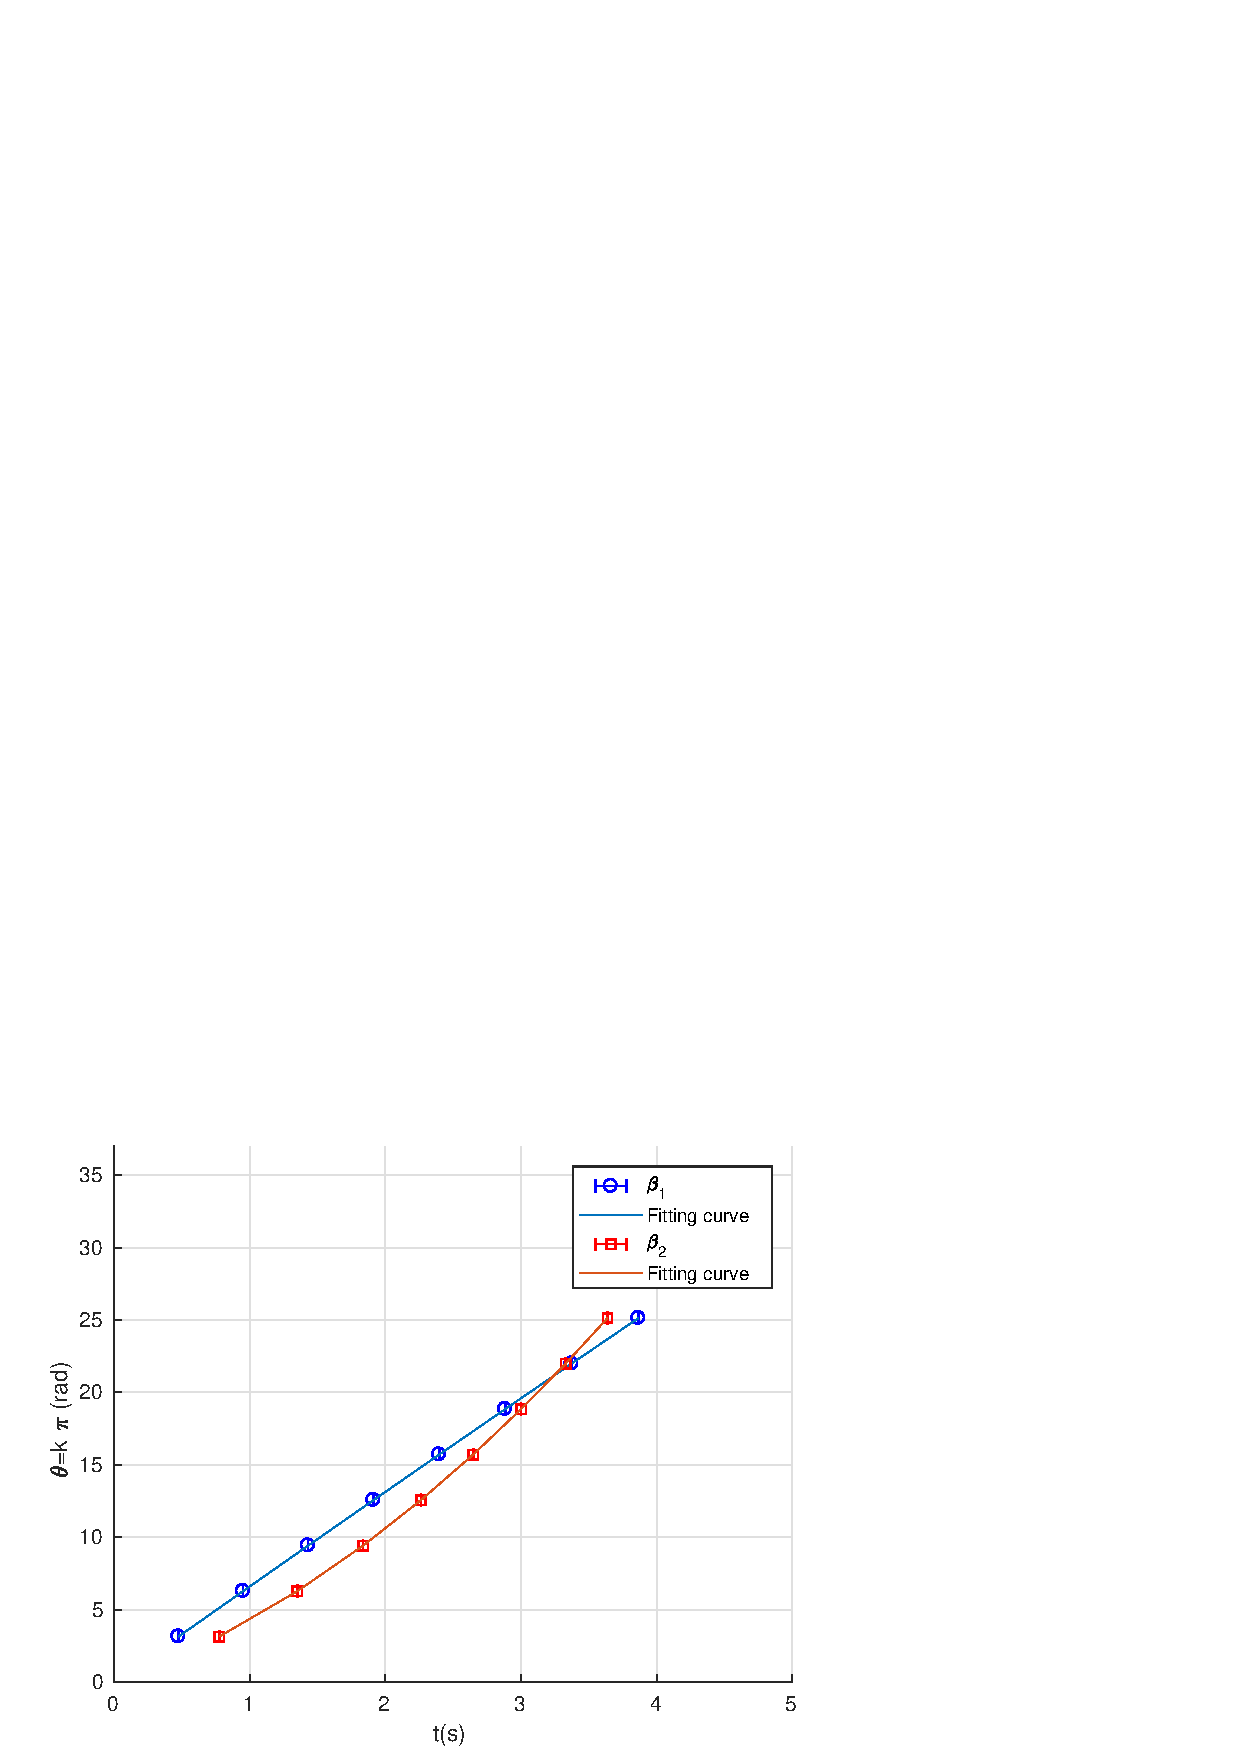
\includegraphics[width=0.8\linewidth]{images/1.png}
        \caption{Stokes’ viscosity measurement apparatus}
        \label{apparatus}
    \end{figure}

    The micrometer is used to measure the diameters of the balls, allowing measurements with maximum uncertainty of $0.004mm$. The calliper is used to measure the inner diameter of the flask, whose maximum uncertainty is $0.02mm$.The densimeter's maximum uncertainty is $0.001 g/cm^3$. The electronic scales' maximum uncertainty is $0.001g$. The stopwatch's maximum uncertainty is $0.01s$. The thermometer's maximum uncertainty is $\SI{2}{\degreeCelsius}$.\\
\section{Measurement Procedure}
\begin{enumerate}
    \item Measure the mass of the weight, the hoop, the disk and the cylinder, as well as the radius of the cone pulley and the cylinder (following the instructor's requirements). Calculate the moment of inertia of the hoop and the disk analytically.\\
    Use a reliable source to find the local value of the acceleration due to gravity in Shanghai.
    \item Turn the electronic timer on and switch it to mode 1-2 (single gate, multiple pulses).
    \item Place the instrument close to the edge of the desk and stretch the disk pulley arm outside so that the weight can move downwards unobstructed.
    \item Level the turntable with bubble level.
    \item Make the turntable rotating and press the start button on the timer. After at least 8 signals are recorded, stop the turntable and record the data in your data sheet.
    \item Attach the weight to one end of the string. Place the string on the disk pulley, thread through the hole in the arm, and wind the string around the third ring of the cone pulley. Adjust the arm holder so that the string goes through the center of the hole.
    \item Release the weight and the start the timer. Stop the turntable when the weight hits the floor. Write down the recorded data.
    \item The angular acceleration can be found by plotting $\theta=k\pi$ against $t$ and performing a quadratic fit using data processing software. (The magnitude of the angular acceleration is equal to the coefficient next to $t^2$ multiplied by two. The uncertainty of the angular acceleration can be read directly from the fitting result.)
\end{enumerate}
\section{Results}
    The frequency we read from the signal generator is $f=35000\pm 1$Hz. The temperature is $24\pm1\SI{}{\degreeCelsius}$.
\subsection{Measurements for resonance method}
    The measurements are shown in Table \ref{data_res} with the calculation for $L_{10+i}-L_i$.
    \begin{table}[h] \small
        \centering
        \begin{tabular}{|c|c|c|c|c|c|}
        \hline
            \multicolumn{2}{|c|}{$L_i[\e{-3}m]\pm[0.01\e{-3}m]$} & 
            \multicolumn{2}{|c|}{$L_i[\e{-3}m]\pm[0.01\e{-3}m]$} &
            \multicolumn{2}{|c|}{$L_{10+i}-L_i[\e{-3}m]$}\\\hline
            1 & 9.90 & 11 & 60.08 & 1 & 50.18 \\\hline
            2 & 14.92 & 12 & 65.08 & 2 & 50.16 \\\hline
            3 & 19.97 & 13 & 70.06 & 3 & 50.09 \\\hline
            4 & 25.02 & 14 & 75.02 & 4 & 50.00 \\\hline
            5 & 30.03 & 15 & 80.25 & 5 & 50.22 \\\hline
            6 & 35.06 & 16 & 85.24 & 6 & 50.18 \\\hline
            7 & 40.03 & 17 & 90.24 & 7 & 50.21 \\\hline
            8 & 45.08 & 18 & 95.22 & 8 & 50.14 \\\hline
            9 & 49.95 & 19 & 100.13 & 9 & 50.18 \\\hline
            10 & 55.01 & 20 & 105.24 & 10 & 50.23 \\\hline
        \end{tabular}
        \caption{Data for the resonance method}\label{data_res}
    \end{table}
    The average value of $\Delta L$ is calculated  based on the results presented in Table \ref{data_res} as
    \[
        \overline{\Delta L}=\frac{1}{10}\sum_{i=1}^{10}\Delta L_i=(50.16\pm 0.05)\e{-3}m,\quad u_{r,\Delta L}=0.10\%.
    \]
    Hence, the wavelength $\lambda$ can be calculated as
    \[
        \lambda=\frac{2\Delta L}{n}=\frac{2\times50.16\e{-3}}{10}=(10.03\pm0.01)\e{-3}m,\quad u_{r,\lambda}=0.10\%.
    \]
    The speed of sound in air $v$ is
    \[
        v=351.05\pm0.4 m/s,\quad u_{r,v}=0.10\%.
    \]

\subsection{Measurements for phase comparison method}
    The measurements are shown in Table \ref{data_pha} with the calculation for $L_{6+i}-L_i$.
    \begin{table}[h] \small
        \centering
        \begin{tabular}{|c|c|c|c|c|c|}
        \hline
            \multicolumn{2}{|c|}{$L_i[\e{-3}m]\pm[0.01\e{-3}m]$} & 
            \multicolumn{2}{|c|}{$L_i[\e{-3}m]\pm[0.01\e{-3}m]$} &
            \multicolumn{2}{|c|}{$L_{6+i}-L_i[\e{-3}m]$}\\\hline
            1 & 54.00 & 7 & 113.41 & 1 & 59.41 \\\hline
            2 & 64.06 & 8 & 122.04 & 2 & 57.98 \\\hline
            3 & 72.97 & 9 & 131.76 & 3 & 58.79 \\\hline
            4 & 81.02 & 10 & 141.83 & 4 & 60.81 \\\hline
            5 & 91.17 & 11 & 153.65 & 5 & 62.46 \\\hline
            6 & 103.49 & 12 & 163.08 & 6 & 59.59 \\\hline
        \end{tabular}
        \caption{Data for the phase comparison method}\label{data_pha}
    \end{table}
    The average value of $\Delta L$ is calculated  based on the results presented in Table \ref{data_res} as
    \[
        \overline{\Delta L}=\frac{1}{6}\sum_{i=1}^{6}\Delta L_i=(59.84\pm 1.7)\e{-3}m,\quad u_{r,\Delta L}=3\%.
    \]
    Hence, the wavelength $\lambda$ can be calculated as
    \[
        \lambda=\frac{\Delta L}{n}=\frac{\times59.84\e{-3}}{6}=(9.973\pm0.3)\e{-3}m,\quad u_{r,\lambda}=3\%.
    \]
    The speed of sound in air $v$ is
    \[
        v=348.95\pm10 m/s,\quad u_{r,v}=3\%.
    \]
\subsection{Measurements for time difference method (liquid)}
    We obtain the speed of sound in water from Table \ref{data_tim} by linear fitting (See Figure \ref{lt}).
    \begin{table}[H] \small
        \centering
        \begin{tabular}{|c|c|c|c|c|}
        \hline
            & $t_i[\e{-6}s]$ & $u_{t_i}[\e{-6}s]$ & $L_i[\e{-3}m]$ & $u_{L_i}[\e{-3}m]$\\\hline
            1 & 159.6 & 0.2 & 230.00 & 0.01\\\hline
            2 & 154.4 & 0.2 & 220.00 & 0.01\\\hline
            3 & 148.2 & 0.2 & 210.00 & 0.01\\\hline
            4 & 141.8 & 0.2 & 200.00 & 0.01\\\hline
            5 & 134.0 & 0.2 & 190.00 & 0.01\\\hline
            6 & 128.0 & 0.2 & 180.00 & 0.01\\\hline
            7 & 121.4 & 0.2 & 170.00 & 0.01\\\hline
            8 & 114.4 & 0.2 & 160.00 & 0.01\\\hline
            9 & 108.0 & 0.2 & 150.00 & 0.01\\\hline
            10 & 101.6 & 0.2 & 140.00 & 0.01\\\hline
            11 & 94.8 & 0.2 & 130.00 & 0.01\\\hline
            12 & 87.8 & 0.2 & 120.00 & 0.01\\\hline
        \end{tabular}
        \caption{Data for Figure \ref{lt}}\label{data_tim}
    \end{table}
    \begin{figure}[H]
        \centering
        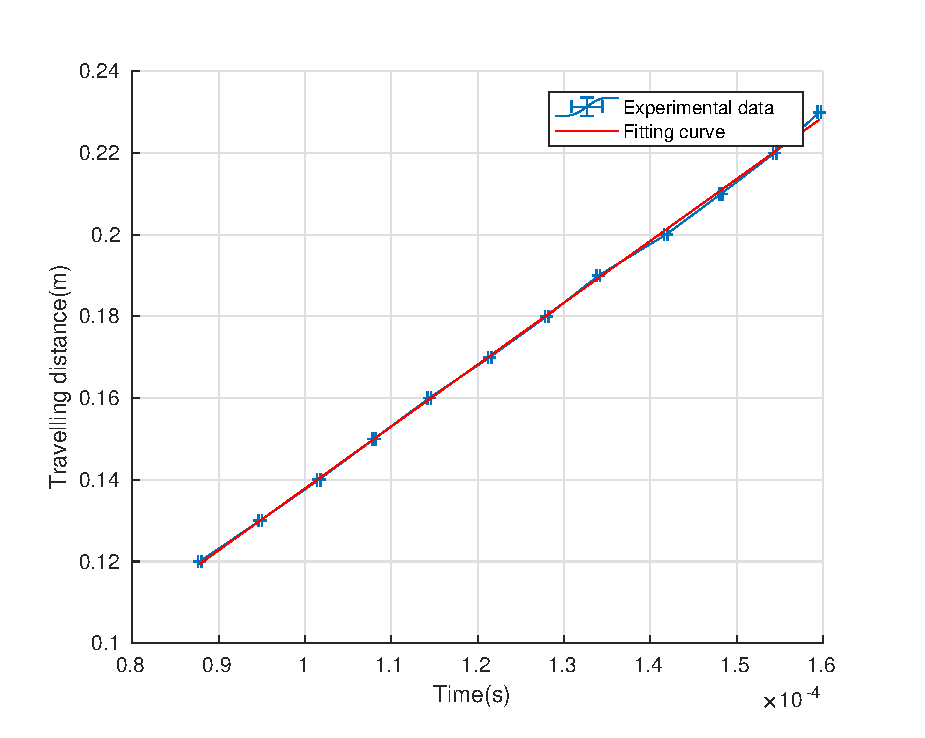
\includegraphics[height=10cm]{images/lt.eps}
        \caption{Fitting curve for $L\ vs.\ t$. (The errorbar is relatively \textbf{small})}\label{lt}
    \end{figure}
    \begin{figure}[H]
        \centering
        \includegraphics[height=6cm]{images/ltinfo.png}
        \caption{Information for Fitting curve in Figure \ref{lt}}\label{ltinfo}
    \end{figure}

    From the data processing of Matalb we know about the slope that 
    \[
        v_{water}=1515\pm20m/s.
    \]
\section{Measurement Uncetainty Analysis}
\subsection{Uncertainty for distances}
    For the calliper measurements except that diameters of holes, we have four measurements for each quantity. To demonstrate the uncertainty, the \textbf{sample calculation} for diameters of the disk will be presented. (raw data see Table \ref{table_calliper})
    \[
    \begin{split}
        &\bar{\varnothing}=0.23992m\\
        &\overline{s_{\varnothing}}=\sqrt{\frac{1}{4(4-1)}\sum_{i=1}^4(\varnothing_i-\bar{\varnothing})^2}\\
        &=\sqrt{\frac{( 0.23994-0.23992)^2+(0.23990-0.23992)^2+(0.23992-0.23992)^2+(0.23992-0.23992)^2}{12}}\\
        &=8.1650\e{-6}m.\\
    \end{split}
    \]
    Then, we obtain the type-A uncertainty and type-B uncertainty respectively. Their square root of sum of squre contribute to the combined uncertainty.
    \[
    \begin{split}
        &t_{0.95}=3.18,\quad n=4,\\
        &\Delta_{A,\varnothing}=t_{0.95}\times\overline{s_{\varnothing}}\approx3\e{-5}m,\\
        &\Delta_{B,\varnothing}=2\e{-5}m,\\
        &u_{\varnothing}=\sqrt{\Delta_{A,\varnothing}^2+\Delta_{B,\varnothing}^2}=\sqrt{(3\e{-5})^2+(2\e{-5})^2}=3\e{-5}m,\\
        &u_{\varnothing,r}=\frac{u_{\varnothing}}{\varnothing}\times100\%=\frac{3\e{-5}}{0.23992}\times100\%=0.014\%
    \end{split}
    \]
    Hence, 
    \[
        \varnothing=0.23992\pm0.00003m,\quad u_{\varnothing,r}=0.014\%.
    \]
    Similarly, we are capable of calculating all the uncertainties (see Table \ref{data_diameter}).

    Then, for the uncertainty of distance from the rotating axis to the holes, we need to calcualte the propagated uncertainty. Here's the \textbf{sample calculation} for hole 1.
    \[
    \begin{split}
        &R_1=\frac{d_{1,in}+d_{1,out}}{2},\\
        &\frac{\partial R_1}{\partial d_{1,in}}=\frac{\partial R_1}{\partial d_{1,out}}=\frac{1}{2},\\
        &u_{d_{1,in}}=u_{d_{1,out}}=\Delta_{dev}=2\e{-5}m\\
        &u_{R_1}=\sqrt{(\frac{\partial R_1}{\partial d_{1,in}})^2(u_{d_{1,in}})^2+(\frac{\partial R_1}{\partial d_{1,out}})^2(u_{d_{1,out}})^2}\\
        &=\sqrt{\frac{1}{4}(2\e{-5})^2+\frac{1}{4}(2\e{-5})^2}=1.4\e{-5}m,\\
        &u_{R_1,r}=\frac{u_{R_1}}{R_1}\times100\%=\frac{1.4\e{-5}}{0.04505}=0.03\%
    \end{split}
    \]

    Hence, 
    \[
        R_1=0.04505\pm 0.00001m,\quad u_{R_1,r}=0.03\%.
    \]

    Similarly, we obtain all the uncertainties of distances between holes (see Table \ref{data_hole}).

\subsection{Uncertainty of mass measurements}
    \textbf{For example}, for the mass of the disk, its uncertainty is merely its type-B uncertainty.
    \[
    \begin{split}
        &u_{m_{disk}}=\Delta_{B}=1\e{-4}kg,\\
        &u_{m_{disk},r}=\frac{u_{m_{disk}}}{m_{disk}}\times100\%=0.02\%
    \end{split}
    \]
    All the uncertainties of mass between holes (see Table \ref{data_mass}).

\subsection{Uncertainty of angular acceleration}
    We will calculate the uncertainty of quadratic fitting by $u=t_{0.95}\cdot std/\sqrt{8-2}$, where $t_{0.95}=2.36$ for n=8. Hoever, the angular acceleration is twice of coefficient of quadratic item. \textbf{For example}, when $p_1=-0.03547\pm0.00099 rad/s^2$ ($p_1$ is the coefficient of quadratic item),
    \[
    \begin{split}
        &\beta=2p_1=2\times (-0.03547)=-0.071rad/s^2,\\
        &u_{\beta}=\sqrt{(\frac{\partial \beta}{\partial p_1})^2(u_{p_1})^2}=2u_{p_1}=0.002rad/s^2,\\
        &u_{\beta,r}=\frac{u_{\beta}}{\beta}\times100\%=\frac{0.002}{0.071}=3\%.
    \end{split}
    \]

    Similar calculation results are listed in Table \ref{data_1}, \ref{data_2}, \ref{data_3}, \ref{data_4}, \ref{data_5}.

\subsection{Uncertainty of the moment of inertia}
    According to Eq. \ref{equ_I}, we know that the uncertainty of the moment of inertia obtains propagated uncertainty.

    Here we have the \textbf{sample calcultion} for empty turntable.
    \[
    \begin{split}
        &\frac{\partial I_1}{\partial m}=\frac{R(g-R\beta_2)}{\beta_2-\beta_1},\\
        &\frac{\partial I_1}{\partial R}=\frac{mg-2mR\beta_2}{\beta_2-\beta_1},\\
        &\frac{\partial I_1}{\partial \beta_1}=\frac{mR(g-R\beta_2)}{(\beta_2-\beta_1)^2},\\
        &\frac{\partial I_1}{\partial \beta_2}=-\frac{mR(R\beta_1+g)}{(\beta_2-\beta_1)^2},\\
        \end{split}
    \]

    \[
    \begin{split}
        u_{I_1}&=\sqrt{(\frac{\partial I_1}{\partial m})^2(u_m)^2+(\frac{\partial I_1}{\partial R})^2(u_R)^2+(\frac{\partial I_1}{\partial \beta_1})^2(u_{\beta_1})^2+(\frac{\partial I_1}{\partial \beta_2})^2(u_{\beta_2})^2}\\
        &=\sqrt{(\frac{R(g-R\beta_2)}{\beta_2-\beta_1})^2(u_m)^2+(\frac{mg-2mR\beta_2}{\beta_2-\beta_1})^2(u_R)^2+(\frac{mR(g-R\beta_2)}{(\beta_2-\beta_1)^2})^2(u_{\beta_1})^2+(-\frac{mR(R\beta_1+g)}{(\beta_2-\beta_1)^2})^2(u_{\beta_2})^2}\\
        &=\sqrt{(0.130)^2(0.0001)^2+(0.280)^2(0.00003)^2+(0.004)^2(0.002)^2+(-0.004)^2(0.012)^2}\\
        &\approx5\e{-5}kg\cdot m^2.\\
        u_{I_1,r}&=\frac{u_{I_1}}{I_1}\times100\%=\frac{0.00005}{0.00707}=0.7\%.
    \end{split}
    \]

    Hence,
    \[
        I_1=(7.07\pm 0.05) \e{-3}kg\cdot m^2, \quad u_{I_1,r}=0.7\%.
    \]

    Simlarly, we can calculate uncertainties for the other combined moments of inertia (see Table \ref{data_I}).

    Finally, due to the additivity of the moment of inertia, we calculate the difference. We take the disk as the \textbf{example}.
    \[
    \begin{split}
        &I_{disk}=I_2-I_1,\\
        &\frac{\partial I_{disk}}{\partial I_2}=1,\\
        &\frac{\partial I_{disk}}{\partial I_1}=-1,\\
        &u_{I}=\sqrt{(\frac{\partial I_{disk}}{\partial I_2})^2(u_{I_2})^2+(\frac{\partial I_{disk}}{\partial I_1})^2(u_{I_1})^2}\\
        &=\sqrt{(3\e{-5})^2+(5\e{-5})^2}\approx0.06\e{-3}kg\cdot m^2.
    \end{split}
    \]

    Simlarly, we can calculate uncertainties for the other moments of inertia (see Table \ref{data_i}).
\section{Conclusions and discussion}
    In this experiment the viscosity coefficient $\eta$ is measured by Stokes' method. We obtain the density of the metal balls by measuring its diameter and mass. We obtain the constant velocity from the traveling distance and time. We measure the inner diameter of the flask and the read the density of castor oil. Finally, the experimentally found $\eta$ of castor oil in the environment of $\SI{24}{\degreeCelsius}, 1 atm$ is
    \[
        \eta=0.679\pm 0.03\frac{kg}{m\cdot s}, \quad u_{r_{\eta}}=3.91\%.
    \]

    After the experiment, I find there are some operations probably leading to deviations in the fundamental Stokes' method. Firstly, I find it hard to confirm that the two beams are parallel. It'll be better if there exist a fixed equipment to measure the distance between the transmitting and the receiving end. Secondly, I find that among the directly measured data, the relative uncertainty of traveling time is the biggest. Stopwatch is indeed not accurate enough to eliminate the deviation. Therefore,the results can be more accurate if the time is recorded by computer when the ball blocks the beams.
\begin{thebibliography}{99}
    \bibitem{foo1} \textsc{Qin} Tian, \textsc{Zeng} Ming, \textsc{Cao} Jianjun, \textsc{Han} Xugen, \textsc{Feng} Yaming, Mateusz \textsc{Krzyzosiak}, Physics Laboratory (Vp141/Vp241) Student Handbook Introduction to Measurement Data Analysis.
    \bibitem{foo2} \text{Qin} Tian, \text{Feng} Yaming, Mateusz \textsc{Krzyzosiak} Physics Laboratory Vp141 Exercise 2 Measurement of Fluid Viscosity.
\end{thebibliography}

\end{document}